\documentclass[12pt,addpoints]{exam}

%Bring in the packages I'll need normally
\usepackage{amsmath} %AMS Math Package
\usepackage{amssymb} %Math symbols like \mathbb
\usepackage{multicol} % Allows for multiple columns
\usepackage{graphicx} %Allows images to be inserted using \includegraphics
\usepackage{enumitem} %Allows for fancier lists, use [noitemsep] or [noitemsep, nolistsep] after \begin{}
\usepackage{hyperref} %Allows the use of web links (\url, \href) and computer paths (\path)

\usepackage{listings} %Way to typeset code; listings respect whitespace. Can be set inline with {\lstinline[breaklines=true]||} or as an environment
\lstset{basicstyle=\ttfamily} %Causes the code environments to be typeset with a Courier-like font

\usepackage[version=3]{mhchem} %Simpler chemistry notation, use \ce{} to typeset chemical formula
	%e.g. \ce{H2O} for water and \ce{1/2SO4^2-} to set half a mol of sulfate ion.

%Set the page to be letter sized with 1" margins
\usepackage[dvips,letterpaper,margin=1in]{geometry}

% See https://www.sharelatex.com/learn/Typing_exams_in_LaTeX
\usepackage{tabularx}
\newcolumntype{Y}{>{\centering\arraybackslash}X}

\rhead{\textbf{Prelistening survey}}
\lhead{\textbf{Sonification of \ce{NO2} trends}}
\headrule

\begin{document}

\renewcommand{\questionshook}{\setlength{\itemsep}{1in}}

\newcommand{\fiveptincdec}{%
\begin{center}
\begin{tabularx}{\textwidth}{YYYYY}
$\square$ & $\square$ & $\square$ & $\square$ & $\square$ \\
Strongly decreasing & Weakly decreasing & No noticeable change & Weakly increasing & Strongly increasing
\end{tabularx}
\end{center}
}

\newcommand{\fiveptmag}{%
\begin{center}
\begin{tabularx}{\textwidth}{YYYYY}
$\square$ & $\square$ & $\square$ & $\square$ & $\square$ \\
Much less & Slightly less & No difference & Slightly greater & Much greater
\end{tabularx}
\end{center}
}

\newcommand{\fiveptgeneric}[2]{%
\begin{center}
\begin{tabularx}{\textwidth}{YYYYY}
1 & 2 & 3 & 4 & 5 \\
$\square$ & $\square$ & $\square$ & $\square$ & $\square$ \\
#1 & & & & #2
\end{tabularx}
\end{center}
}

\begin{questions}


\question \ce{NO2} from cities:
	\begin{parts}
	\part Do you expect the overall trend in US cities' \ce{NO2} to be increasing, decreasing, or staying constant over the time period from 2005 to 2015?
	\fiveptincdec

	\part Rate your confidence in this answer.
	\fiveptgeneric{Minimal confidence}{Extremely confident}
	\end{parts}


\question \ce{NO2} from power plants:
	\begin{parts}
	\part Do you expect the overall trend in power plants' \ce{NO2} to be increasing, decreasing, or staying constant over the time periods from 2005 to 2015?
	\fiveptincdec

	\part Rate your confidence in this answer.
	\fiveptgeneric{Minimal confidence}{Extremely confident}
	\end{parts}


\question \ce{NO2} in rural areas:
	\begin{parts}
	\part Do you expect the overall trend in rural locations' \ce{NO2} to be increasing, decreasing, or staying constant over the time period 2005 to 2015?
	\fiveptincdec
	
	\part Rate your confidence in this answer.
	\fiveptgeneric{Minimal confidence}{Extremely confident}
	\end{parts}


\question Seasonal variation:
	\begin{parts}
	\part Do you expect the amount of \ce{NO2} in the summer to be greater or less than in the winter, in general?
	\fiveptmag

	\part Rate your confidence in this answer.
	\fiveptgeneric{Minimal confidence}{Extremely confident}
	\end{parts}
	
\question Spatialization:
	\begin{parts}
	\part Which city would you expect to have the largest change in \ce{NO2}? \\
		\begin{choices}
		\choice Indianapolis
		\choice Los Angeles, CA
		\choice Reno, NV
		\choice San Antonio, TX
		\end{choices}
		
		\part Rate your confidence in this answer.
		\fiveptgeneric{Minimal confidence}{Extremely confident}
		
	\end{parts}

\question Regional trends:
	\begin{parts}
	\part Which region do you expect had the greatest \ce{NO2} in 2005?\\
		\begin{choices}
		\choice Northeast
		\choice Southeast
		\choice Northwest
		\choice Southwest
		\end{choices}
		
		\part Rate your confidence in this answer.
		\fiveptgeneric{Minimal confidence}{Extremely confident}
	\end{parts}
	
\question \ce{NO2} at rural sites:
	\begin{parts}
	\part This interface includes \ce{NO2} from 15 rural sites, shown in the image below.  Which two do you expect would have the greatest change in \ce{NO2} from 2005 to 2015?

	\makeemptybox{1cm}
	
	\begin{center}
	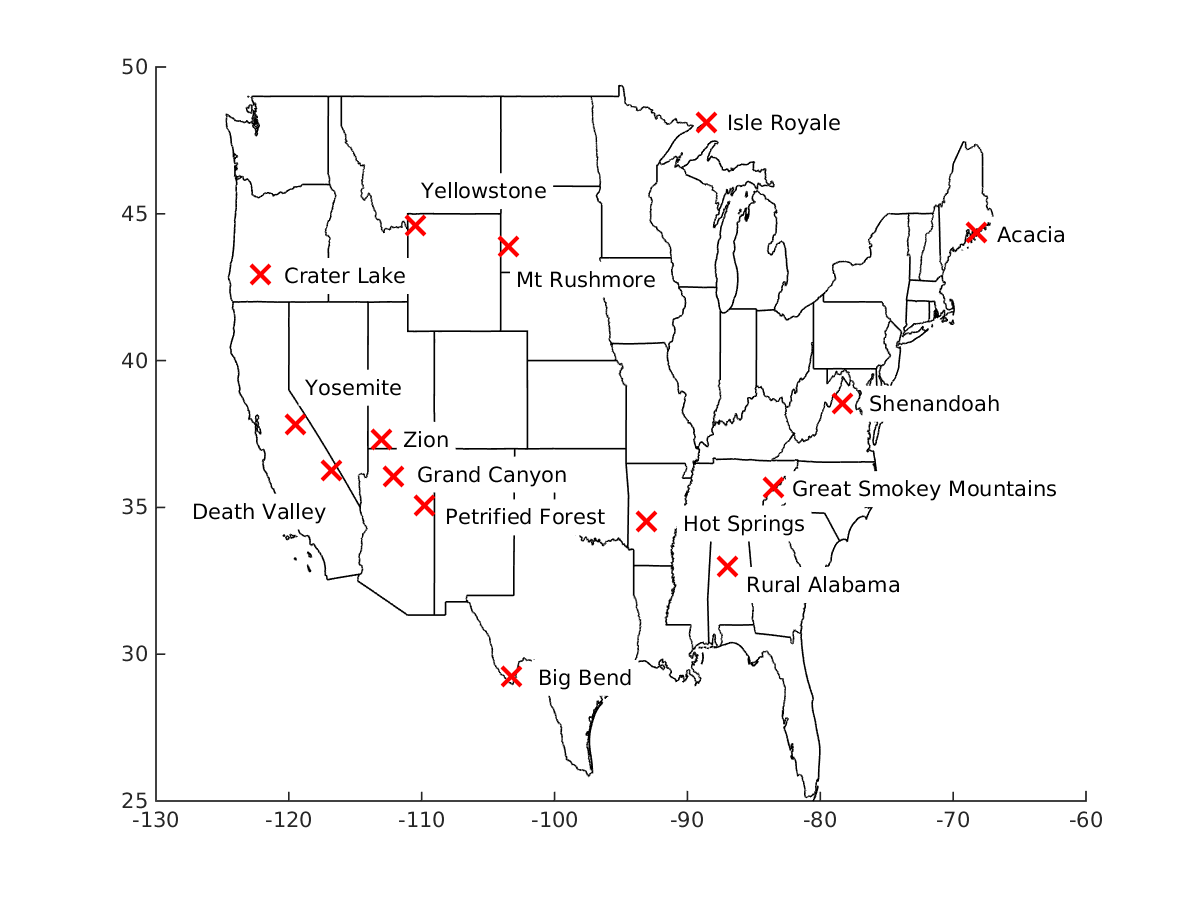
\includegraphics[width=0.75\textwidth]{Images/rural-sites.png} 	
	\end{center}
	


	\end{parts}
\end{questions}

\end{document}
